\section{Условие}

Необходимо для сложной системы $S$, имеющей не более 10 состояний, определить среднее время нахождения системы в предельных состояниях, то есть при установившемся режиме работы. На вход подается матрица, на пересечении строк и столбцов которой находится интенсивность перехода.

\section{Теория}

По модели из условия строятся уравнения Колмогорова: в левой части уравнений находится производная вероятности состояний, а правая часть содержит члены по количеству переходов, связанных с текущим состоянием. Если направление перехода в текущее состояние, то соответствующий член имеет знак минус, если направление из состояния, то плюс. Каждый член равен произведению плотности вероятности перехода на вероятость того состояния, из которого идет этот переход.

Поскольку модель имеет установившийся режим, то левые части уравненя будут равно нулю. Далее вводится уравнение нормировки и производится подсчет.

Получившиеся вероятности являются средним относительным временем пребывания системы в данном состоянии.

Среднее время находится по формуле \ref{eq:time}

\begin{equation}\label{eq:time}
    t_i = \frac{1 - p_i}{p_i \cdot \sum_{i \ne j}\lambda_{ij}}
\end{equation}

\section{Результаты}

На рисунках \ref{fig:4}, \ref{fig:5} и \ref{fig:6} представлены результаты работы для систем из 4, 5 и 6 состояний соотвественно.

\begin{figure}[H]
    \centering
    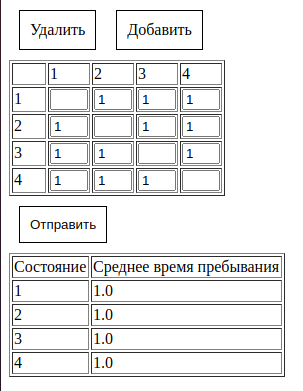
\includegraphics[width=0.4\textwidth]{img/content/4.png}
    \caption{4 состояния}
    \label{fig:4}
\end{figure}

\begin{figure}[H]
    \centering
    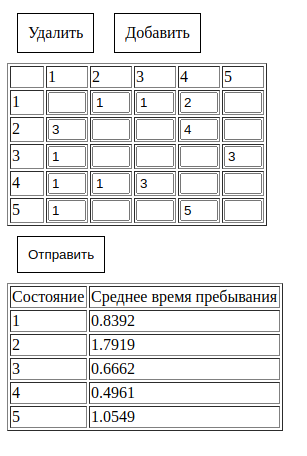
\includegraphics[width=0.4\textwidth]{img/content/5.png}
    \caption{5 состояний}
    \label{fig:5}
\end{figure}

\begin{figure}[H]
    \centering
    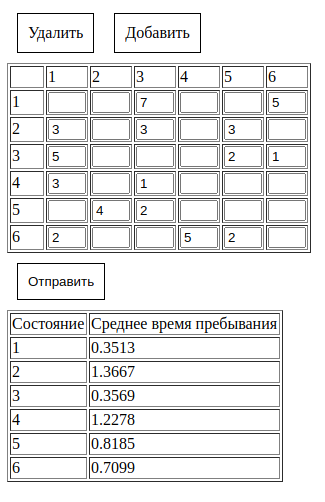
\includegraphics[width=0.4\textwidth]{img/content/6.png}
    \caption{6 состояний}
    \label{fig:6}
\end{figure}

\section{Вывод}

Была разработана программа, которая для сложной системы $S$, имеющей не более 10 состояний, определяет среднее время нахождения системы в предельных состояниях, то есть при установившемся режиме работы.
